\documentclass [11pt,twoside]{article}
\usepackage[utf8]{inputenc}
\usepackage[T1]{fontenc}
\usepackage{import}
\documentclass [11pt,twoside]{article}
\usepackage[utf8]{inputenc}
\usepackage[T1]{fontenc}

%Page margins, header and footer positions
\usepackage{geometry}
 \geometry{
 a4paper,
 % total={210mm,297mm},
 left=25mm,
 right=25mm,
 top=30mm,
 bottom=25mm,
 headsep=7mm}

\interfootnotelinepenalty=10000

%To display filling dots in the TOC for all entries
\usepackage[titles]{tocloft}
\renewcommand{\cftsecleader}{\cftdotfill{\cftdotsep}}

%Define new header and footer style
\usepackage{fancyhdr}

\pagestyle{fancy}
\fancyhf{}
\lhead{\color{Gray}{\small{Travlendar+ project by YOUR NAMES}}}
\lfoot{\textcolor{Gray}{\small{Copyright © 2017, YOUR NAMES – All rights reserved}}}
\rfoot{\textcolor{Gray}{\thepage}}
\renewcommand{\headrulewidth}{0pt}

%PACKAGES
\usepackage{wasysym}
\usepackage{pifont}

\newcommand{\supported}{\ding{52}\xspace}
\newcommand{\unsupported}{\ding{55}\xspace}
\newcommand{\partsupported}{\textcolor{black!40}{\ding{52}}\xspace}
\newcommand{\lowsupported}{\textcolor{black!20}{\ding{52}}\xspace}
\newcommand{\unknowsupported}{\textbf{?}\xspace}

%Font: Times
\usepackage{times}
%Change monospaced font
\renewcommand{\ttdefault}{lmtt}

%tables
%\usepackage{tabu}
\usepackage{tabularx}
\usepackage{ltablex}
\usepackage{longtable}
\usepackage{float} % To allow the use of H modifier in long tables

%landscape mode
\usepackage{pdflscape}
\usepackage{rotating}
\usepackage{caption}

%make landscape mode be sensitive to even and odd pages
%start
\def\myrotate{\ifodd\c@page\else-\fi 90}
\makeatletter
\global\let\orig@begin@landscape=\landscape%
\global\let\orig@end@landscape=\endlandscape%
\gdef\@true{1}
\gdef\@false{0}
\gdef\landscape{%
    \global\let\within@landscape=\@true%
    \orig@begin@landscape%
}%
\gdef\endlandscape{%
    \orig@end@landscape%
    \global\let\within@landscape=\@false%
}%
\@ifpackageloaded{pdflscape}{%
    \gdef\pdf@landscape@rotate{\PLS@Rotate}%
}{
    \gdef\pdf@landscape@rotate#1{}%
}
\let\latex@outputpage\@outputpage
\def\@outputpage{
    \ifx\within@landscape\@true%
        \if@twoside%
            \ifodd\c@page%
                \gdef\LS@rot{\setbox\@outputbox\vbox{%
                    \pdf@landscape@rotate{-90}%
                    \hbox{\rotatebox{90}{\hbox{\rotatebox{180}{\box\@outputbox}}}}}%
                }%
            \else%
                \gdef\LS@rot{\setbox\@outputbox\vbox{%
                    \pdf@landscape@rotate{+90}%
                    \hbox{\rotatebox{90}{\hbox{\rotatebox{0}{\box\@outputbox}}}}}%
                }%
            \fi%
        \else%
            \gdef\LS@rot{\setbox\@outputbox\vbox{%
                \pdf@landscape@rotate{+90}%
                \hbox{\rotatebox{90}{\hbox{\rotatebox{0}{\box\@outputbox}}}}}%
            }%
        \fi%
    \fi%
    \latex@outputpage%
}
\makeatother
%end

%graphics
\usepackage{graphicx}
\usepackage[dvipsnames, table]{xcolor}
%If you upload images from PC, you need to insert code for the path here (different for Windows and Unix OS)

%References
%\usepackage{xpatch}
%\usepackage[backend=biber, style=numeric, citestyle=numeric, sorting=none]{biblatex}
%\addbibresource{main.bib}

%Other
\usepackage{ifthen}
\usepackage{xspace}
\usepackage{enumitem}
\usepackage{amssymb}
\usepackage[pdftex, colorlinks]{hyperref}
\newcommand{\comment}[1]{{\color{Red}$\blacktriangleright$ Comment: #1 $\blacktriangleleft$}}


% Some utilities\ldots
\usepackage{soul}
\usepackage{tikz}

\usetikzlibrary{calc}
\usetikzlibrary{decorations.pathmorphing}


\makeatletter

\newcommand{\defhighlighter}[3][]{%
  \tikzset{every highlighter/.style={color=#2, fill opacity=#3, #1}}%
}

\defhighlighter{yellow}{.5}

\newcommand{\highlight@DoHighlight}{
  \fill [ decoration = {random steps, amplitude=1pt, segment length=15pt}
        , outer sep = -15pt, inner sep = 0pt, decorate
       , every highlighter, this highlighter ]
        ($(begin highlight)+(0,8pt)$) rectangle ($(end highlight)+(0,-3pt)$) ;
}

\newcommand{\highlight@BeginHighlight}{
  \coordinate (begin highlight) at (0,0) ;
}

\newcommand{\highlight@EndHighlight}{
  \coordinate (end highlight) at (0,0) ;
}

\newdimen\highlight@previous
\newdimen\highlight@current

\DeclareRobustCommand*\highlight[1][]{%
  \tikzset{this highlighter/.style={#1}}%
  \SOUL@setup
  %
  \def\SOUL@preamble{%
    \begin{tikzpicture}[overlay, remember picture]
      \highlight@BeginHighlight
      \highlight@EndHighlight
    \end{tikzpicture}%
  }%
  %
  \def\SOUL@postamble{%
    \begin{tikzpicture}[overlay, remember picture]
      \highlight@EndHighlight
      \highlight@DoHighlight
    \end{tikzpicture}%
  }%
  %
  \def\SOUL@everyhyphen{%
    \discretionary{%
      \SOUL@setkern\SOUL@hyphkern
      \SOUL@sethyphenchar
      \tikz[overlay, remember picture] \highlight@EndHighlight ;%
    }{%
    }{%
      \SOUL@setkern\SOUL@charkern
    }%
  }%
  %
  \def\SOUL@everyexhyphen##1{%
    \SOUL@setkern\SOUL@hyphkern
    \hbox{##1}%
    \discretionary{%
      \tikz[overlay, remember picture] \highlight@EndHighlight ;%
    }{%
    }{%
      \SOUL@setkern\SOUL@charkern
    }%
  }%
  %
  \def\SOUL@everysyllable{%
    \begin{tikzpicture}[overlay, remember picture]
      \path let \p0 = (begin highlight), \p1 = (0,0) in \pgfextra
        \global\highlight@previous=\y0
        \global\highlight@current =\y1
      \endpgfextra (0,0) ;
      \ifdim\highlight@current < \highlight@previous
        \highlight@DoHighlight
        \highlight@BeginHighlight
      \fi
    \end{tikzpicture}%
    \the\SOUL@syllable
    \tikz[overlay, remember picture] \highlight@EndHighlight ;%
  }%
  \SOUL@
}

\makeatother

% Common abbrev. are set as commands to ensure proper spacing after the dot
\RequirePackage{xspace}
\newcommand{\ie}{i.e.\@\xspace}
\newcommand{\aka}{a.k.a.\@\xspace}
\newcommand{\Ie}{I.e.\@\xspace}
\newcommand{\cf}{cf.\@\xspace}
\newcommand{\Cf}{Cf.\@\xspace}
\newcommand{\eg}{e.g.\@\xspace}
\newcommand{\Eg}{E.g.\@\xspace}
\newcommand{\etal}{et al.\@\xspace}
\newcommand{\etc}{etc.\@\xspace}
\newcommand{\wrt}{w.r.t.\@\xspace}
\newcommand{\Wrt}{W.r.t.\@\xspace}



\date{}

%References
\usepackage{xpatch}
\usepackage[backend=biber, style=numeric, sorting=none, defernumbers=true]{biblatex}
\addbibresource{ATD.bib}
\nocite{*}
\DeclareFieldFormat{annotation}{\par\textit{#1}}
\renewbibmacro*{begentry}{\printfield{annotation}}
%%%

\usepackage{fancyhdr}

\pagestyle{fancy}
\fancyhf{}
\lhead{\color{Gray}{\small{ATD by Ricci, Paoli, Grisoni}}}
\lfoot{\textcolor{Gray}{\small{Copyright © 2025, Ricci, Paoli, Grisoni – All rights reserved}}}
\rfoot{\textcolor{Gray}{\thepage}}
\renewcommand{\headrulewidth}{0pt}
%%

\usepackage[dvipsnames]{xcolor}
\usepackage{listings}
\usepackage{alloy-style}
\setlength{\headheight}{13.6pt}

\setcounter{secnumdepth}{5}
\setcounter{tocdepth}{5}  % Includi fino a \paragraph nel sommario

\begin{document}

    %TITLE PAGE
    \begin{titlepage}

        % LOGO e titolo sopra
        \vspace*{-2cm} % (opzionale) aggiusta il margine superiore
        \begin{center}
            \begin{tabularx}{\textwidth}{>{\raggedleft\arraybackslash}p{0.30\textwidth}>{\raggedleft\arraybackslash}X}
                \textcolor{titleColor}{\textbf{\small{ATD Ricci, Paoli, Grisoni}}} & 
\includegraphics[scale=0.5]{Images/PolimiLogo} \\
            \end{tabularx}
        \end{center}
        % Spazio verticale tra logo e titolo
        \vspace*{4cm} % Sostituito \vspace con \vspace* per garantire lo spazio anche all'inizio della pagina
    
        % TITLE
        \begin{center}
            % Titolo del documento
            {\textcolor{titleColor}{\textbf{\Huge{ATD}}}} \\[2ex]
            {\textcolor{titleColor}{\textbf{\Huge{Acceptance Testing Deliverable}}}} \\[1cm]
        \end{center}
    \end{titlepage}
    
    %Define deliverable specific info
    %Replace cell contents where needed
    \begin{table}[h!]
        \renewcommand{\arraystretch}{1}
        \setlength{\extrarowheight}{2pt}
        \begin{tabularx}{\textwidth}{>{\raggedleft\arraybackslash}p{0.3\textwidth}>{\raggedright\arraybackslash}X}
            \hline
            \textbf{Deliverable:} & ATD \\ 
            \textbf{Title:} & Acceptance Testing Deliverable \\ 
            \textbf{Authors:} & Lorenzo Ricci, Matteo Giovanni Paoli, Samuele Grisoni \\ 
            \textbf{Version:} & 1.0 \\ 
            \textbf{Date:} & 09-02-2025 \\ 
            \textbf{Download page:} & \url{https://github.com/Slaitroc/RicciPaoliGrisoni/} \\ 
            \textbf{Copyright:} & Copyright © 2025, Ricci, Paoli, Grisoni – All rights reserved \\ \hline
        \end{tabularx}
    \end{table}
    
  
    
    \setcounter{page}{2}
    %------------------------------------------------------------------------------------------------------------------------------------------------
    \newpage
    \addcontentsline{toc}{section}{Contents}
    \tableofcontents
    \newpage
    \listoffigures
    \newpage

    \listoftables
    %------------------------------------------------------------------------------------------------------------------------------------------------
    \clearpage
    \section{Introduction}
    \label{sect:introduction}
    \subsection{Tested Project}

\begin{itemize}
    \item \textbf{\color{titleColor}Project Name:} 
    \begin{itemize}[label= {\color{titleColor}\(\diamond\)}]
        \item RojasJinLe \(\longrightarrow\) \href{https://github.com/felixsrp/RojasJinLe}{https://github.com/felixsrp/RojasJinLe}
    \end{itemize}
    \item \textbf{\color{titleColor}Authors:} 
    \begin{itemize}[label= {\color{titleColor}\(\diamond\)}]
        \item Felix Rojas
        \item Tai Le
        \item Wenjie Jin
    \end{itemize}
    \item \textbf{\color{titleColor}Reference Documents:}
    \begin{itemize} [label= {\color{titleColor}\(\diamond\)}]
        \item \href{https://github.com/felixsrp/RojasJinLe/blob/a8bf129840a9f7ffc102c44593fcca93a684c4cb/DeliveryFolder/RASDv4.pdf}{RASD}
        \item \href{https://github.com/felixsrp/RojasJinLe/blob/a8bf129840a9f7ffc102c44593fcca93a684c4cb/DeliveryFolder/DDv3.pdf}{DD}
        \item \href{https://github.com/felixsrp/RojasJinLe/blob/a8bf129840a9f7ffc102c44593fcca93a684c4cb/DeliveryFolder/ITDv1.pdf}{ITD}
    \end{itemize}
\end{itemize}

\subsection{Delivered Prototype}
The delivered prototype consists of an Android portable device application that connects to a set of containers responsible for running:
\begin{itemize}[label= {\color{titleColor}\(\diamond\)}]
    \item the Postgres Database;
    \item an SMTP local server for sending email;
    \item Adminer: a service to visualize and handle DB data;
    \item the backend serving the api endpoints. 
\end{itemize}

\subsection{Acronyms, Abbreviations, and Definitions}
Here, we present a table that contains some acronyms and abbreviations along with their definitions, which will be used throughout this document or are defined within the context of the application.
\begin{table}[h!]
    \centering
    \begin{tabular}{|>{\bfseries}c|>{\centering\arraybackslash}p{0.7\textwidth}|}
        \hline
        \textbf{ACRONYM} & Definition \\
        \hline
        \textbf{RASD} & Requirements Analysis and Specification Document \\
        \hline
        \textbf{ITD} & Implementation and Testing Document \\
        \hline
        \textbf{ATD} & Acceptance Test Document \\
        \hline
        \textbf{ECT} & Edge Case Test \\
        \hline
        \textbf{Anomaly} & Unexpected behavior of the application \\
        \hline
        \textbf{Note} & Peculiarities of the functionality and/or design choices \\
        \hline
        \textbf{Skill/Tag} & A keyword that describes an ability of a student or a requirement of a job offer, used in the matching algorithm \\
        \hline
        \textbf{Assigment} & The document that contains the requirements of the project described in a non-formal way\\
        \hline
    \end{tabular}
    \caption{Acronyms}
    \label{tab:definitions}
\end{table}
  
    %------------------------------------------------------------------------------------------------------------------------------------------------
    \clearpage
    \section{Installation}
    \label{sect:installation}
    \subsection{Prerequisites Installation}
The ITD provided by the group under analysis properly covers the installation guide for the software prerequisites.
The software in question is:
\begin{itemize}
    \item Windows Subsystem for Linux 2 (WSL2):\\
         a compatibility layer that enables running a full Linux kernel on Windows. It is needed to be able to install and use the next prerequisite;
    \item Docker Desktop:\\
    an application that enables running and managing Docker containers on Windows, integrating WSL 2 for improved performance and native Linux compatibility.
    \item Node.js:\\
    a JavaScript runtime built on Chrome's V8 engine that allows executing JavaScript code outside the browser, enabling backend development and server-side applications.
\end{itemize}
Since these are very common tools and pieces of software, widely used by developers, their installation was not necessary, as our systems already had them installed and set up.

\subsection{Backend Environment Set Up}

In the \verb|backend| directory, there are all the needed files to properly configure the backend services. The "\verb|docker-compose.yaml|" file defines four services:
\begin{itemize}
    \item Postgres service:\\
        Database;
    \item Adminer service: \\
        Database Manager with UI;
    \item Mail service:\\
        SMTP server for sending email in a dev environment;
    \item API service:\\
        the service responsible to run the node server derving the business logic api.
\end{itemize}

As specified by the ITD, the only services that shall run in separated containers are the first three as the api one shall be run locally, ignoring the docker compose setup defined for it. 



\subsubsection*{Installation Steps}

The steps we executed once in the main project directory are:
\begin{enumerate}
    \item Navigate to the \verb|backend| directory:
        \begin{verbatim}
            cd backend
        \end{verbatim}
\item Install the Node.js project dependencies:
        \begin{verbatim}
            npm install
        \end{verbatim}
\item Run the three docker containers:
        \begin{verbatim}
            docker compose up -d postgres adminer maildev
        \end{verbatim}
The \verb|-d| argument lauch the containers in detached mode meaning the terminal will still be available to run other commands (while by default it keeps showing the docker logs)
\item Install api server dependencies:
        \begin{verbatim}
            npm install
        \end{verbatim}
\item Execute the npm script to construct the database:
        \begin{verbatim}
            npm run migration:run
        \end{verbatim}
\item Seed the database:
        \begin{verbatim}
            npm run seed:run:relational
        \end{verbatim}
\item Start the server locally on our device:
        \begin{verbatim}
            npm run start:dev
        \end{verbatim}
\end{enumerate}

\subsubsection*{Result}
After executing all the previous commands, we have three containers running the following services:
\begin{itemize}
    \item Postgres service:\\
        Database;
    \item Adminer service: \\
        Database Manager with UI;
    \item Mail service:\\
        SMTP server for sending email in a dev environment;
\end{itemize}

\begin{figure}[H]
    \centering
    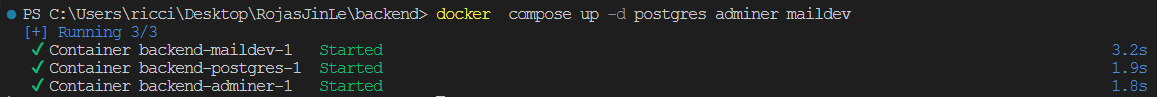
\includegraphics[width=1\linewidth]{Latex/Images/ATD/containers.png}
    \caption{Running Containers}
    \label{fig:containers}
\end{figure}

And the api server running on directly on our device OS ready to serve on \verb|localhost:3000|:

\begin{figure}[H]
    \centering
    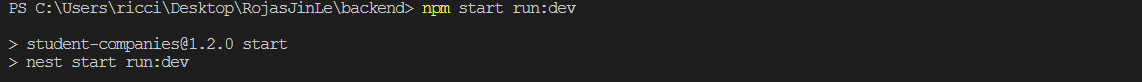
\includegraphics[width=1\linewidth]{Latex/Images/ATD/npmrun.png}
    \caption{Running API server}
    \label{fig:containers}
\end{figure}



\subsection{Frontend Environment Set Up}
As the prototype client is an Android application we need an emulator to be able to test it. The ITD specify to use the Android Studio IDE emulator to run the application; so we installed it on our devices.
The ITD also provided us with a link to a cloud storage containing the build of the client app that we downloaded and copied into the emulator.

\subsubsection*{Installation Steps}
\begin{enumerate}
    \item Install Android Studio IDE from its website;
    \item Create a new android device emulator and start it;
    \item Download the client build file from the cloud storage link;
    \item Copy the build file into the running emulator
    \item Open the client application;
\end{enumerate}

\subsubsection*{Result}
The result is a running portable android device emulator containing the client application ready for testing.


\begin{figure}[H]
    \centering
    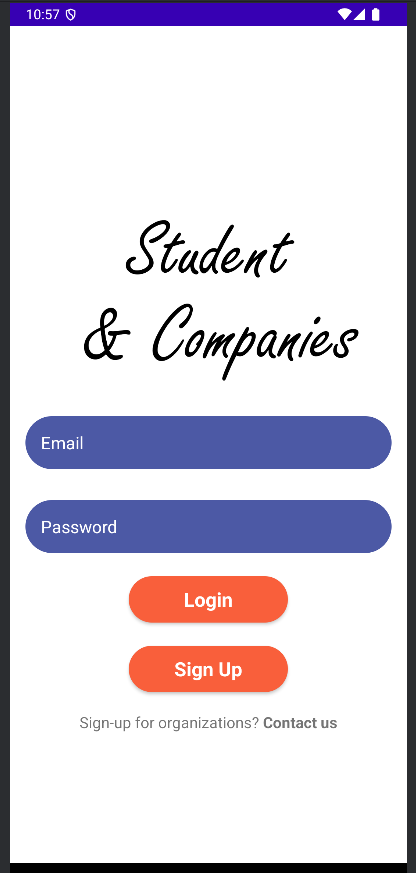
\includegraphics[width=0.3\linewidth]{Latex/Images/ATD/AndroidApp.png}
    \caption{Android Emulator running the client App}
    \label{fig:androidapp}
\end{figure}




 
    %------------------------------------------------------------------------------------------------------------------------------------------------

    %  \clearpage
    % \section{Old Tests section}
    % \label{sect:oldtest}
    % \subsubsection{Signup, CV upload, Login \& Authorization}
This test concerns user registration on the platform, the CV upload phase, and user session validation through Log In. To check the integration between all the services, we first tested the API endpoints to determine which fields are required in the request body. Then, using the Adminer service, we verified whether the newly created user was correctly inserted into the database. As the final step, we followed the same process using the application. This approach helped us identify weaknesses or inconsistencies in the application. The direct call to the endpoint was easily handled through Postman, thanks to the Postman workspace configuration file provided in the ITD.
\subsubsection*{Steps}
\begin{enumerate}
    \item Postman call to API endpoint \verb|/api/v1/auth/email/register| with the following body:
    \begin{verbatim}
    "email": "teststudent1@mail.com",
    "password": "password",
    "fullName": "Student Test",
    "gender": "Male",
    "phoneNumber": "00000000",
    "aboutYou": "Student looking for an internship",
    "address": "Padova",
    "university": "Test University",
    "personalEmail": "example@personal.com",
    "attributes": "Software Engineering, Python,
                    NodeJs, React, JavaScript, Italian, English",
    "cv": "https://www.cv.com/link",
    "role": 2 // Role is 1 for admin, 2 for student, 3 for company,
                4 for university
    \end{verbatim}
    Result: \verb|204 No Content|\\
    The result shows the server correctly registered the new user of type student.
    \item Postman call to API endpoint \verb|/api/v1/auth/email/login| with body:
    \begin{verbatim}
    "email": "teststudent1@mail.com",
    "password": "password"
    \end{verbatim}
    Result: \verb|200 OK|\\
   The response code and response body show that the user was correctly authenticated. The response body also contains the new user's information and the necessary tokens (token and refresh token) to handle user session validation.
    \item Database check:\\
    Using Adminer, we checked the tables that handle the new data. The newly created user data is present and correctly inserted into the database, confirming the proper integration of all the services under analysis.
    \item Frontend application sign up process:\\
    Using the client application, we proceeded with the same actions, meaning we attempted to register the same user. First, we inserted all the required data. As specified in the ITD, there is no validation on the input sent by the user, as the platform assumes it to be correct. Then, we uploaded the CV file, which is handled as a link in the respective API call.

    To upload the CV file, we used the Android device emulator's file system. We were able to copy a mock-up file into the emulator and then upload it to the app thanks to the provided file system interface. Additionally, we selected relevant skills from a predefined set for our test student and were also able to add custom skills.

    However, after pressing the Sign Up button, the client app allowed us to create the same user twice, which should not be allowed.
    
    \item Database check:\\
    Checking the database, we observed that the user was neither created twice nor updated, as the creation date remained the same as the previous entry.
    \item Postman call to the API endpoint \verb|/api/v1/auth/email/register| using the same request body as in step one.\\
    Result: \verb|422 Unprocessable Entity|\\
    Body: 
    \begin{verbatim}
    "status": 422,
    "errors": {
        "email": "emailAlreadyExists"
    }
    \end{verbatim}
   Since the API response indicated that it is not possible to create two users with the same email, we assume there is an anomaly in how the frontend application handles this situation.
    
    \item Login using frontend application:\\
    By entering the user’s email and password, the application correctly allowed the student to access the dashboard page.

    \item Postman API Call to endpoints supposed to require the Authorization header:\\
    Despite the fact that the API call for user login responds with the necessary tokens for authorization, it seems that by removing the Authorization header, most of the calls still function as usual, returning information that should require proper authorization.
    
\end{enumerate}

\subsection*{Tested Cases}
\begin{itemize}
    \item Student signup through server API request;
    \item Student signup through frontend application;
    \item Student signup of two users with the same data through frontend application;
    \item CV Upload during registration through frontend application;
    \item Signup of two users with the same data through server API request;
    \item User login through server API request;
    \item User login through frontend application;
    \item Server API calls without Authorization header;
\end{itemize}

\subsubsection*{Result}
\textbf{Partial Success:}
The tests revealed inconsistencies between the frontend and backend. The frontend incorrectly allows duplicate user registrations, displaying a confirmation message despite the API rejecting them. A major security issue was identified: API calls that should require authorization still return data even when the Authorization header is missing. Additionally, the frontend lacks an interface to modify or view uploaded CVs.

\subsubsection*{Anomalies}
\begin{itemize}
    \item The frontend allows duplicate user registrations, confirming them incorrectly, while the API correctly prevents this. This suggests an issue in how the frontend handles API responses.
    \item The CV column in the database stores uploaded files as links, despite the files being provided through the device's file system. This design choice will be further tested.
    \item The aboutYou field is missing in the frontend, as there is no input field for it.
    \item API calls requiring the Authorization header still return sensitive information even when the header is absent, indicating a security risk.
    \item After logging out of the application, if the “go back” gesture is performed on the device, the user is brought back to the previous user account
    
\end{itemize}

\subsubsection*{Notes}
\begin{itemize}
    \item As specified in the ITD, the frontend only handles student registration. Other user types were tested via API calls, which functioned correctly.
    \item The university selection in the frontend includes options not registered on the platform, and newly added universities do not appear in the list. However, custom universities can still be entered manually, so this is not considered an anomaly.
    \item The frontend does not allow users to modify, view, or manage their CVs or personal data.
    \item Expected platform suggestions during registration and CV uploading were missing, despite being included in the prototype description.
\end{itemize}

\subsubsection{Create Internship and Search Internship}
This test concerns internship creation and filtering, which should be based on internship details. The filtering functionality is available on the dashboard page of the frontend application and is accessible to Company and Student user types. Since there are no explicit API calls for this feature, we assume it is implemented directly within the client application.
% qui mi sembra che il problema fosse che in un qualche documento dicono che si basa sulla descrizione e sulla location tipo.
\subsubsection*{Steps}
\begin{enumerate}
    \item Multiple Postman calls to the API endpoint \verb|/api/v1/internships| to create different internships.\\
    Request body:
    \begin{verbatim}
  {
  "company": {
    "id": <id-number>
  },
  "title": <internship-title>,
  "description": <internship-description>,
  "requiredSkills": <internship-reqskills>,
  "optionalSkills": <internship-optskills>,
  "startDate": <internship-startdate>,
  "endDate": <internship-enddate>,
  "duration": <internship-duration>,
  "salary": <internship-salary>,
  "type": <internship-type>
}
    \end{verbatim}
    The calls successfully created the internships.
    
    \item Internship creation using frontend application:\\
    The frontend successfully allows the creation of internships, and database checks confirm the correct execution of the process. However, some fields that could be included in the request body are not handled by the client application. Additionally, for the next steps, it is important to note that each internship inherits its location from the company’s registered location.
    
    \item Available internship filtering based on location:    \\ 
    Since internships inherit their location from the company that owns them, this feature does not seem particularly useful. Additionally, in the client application, selecting a random city for internship filtering returns the same results as applying no filter, indicating that the feature is not correctly implemented.
    
    \item Available internship filtering based on internship data:\\
   This feature only works for filtering by internship title, required skills, and optional skills. However, if a company name or part of the internship description is entered, the filtering fails, indicating incomplete implementation.
    
\end{enumerate}
\subsubsection*{Tested Cases}
\begin{itemize}
    \item Internship creation via API;
    \item Internship creation via frontend;
    \item Location-based filtering;
    \item Internship data filtering;
    
\end{itemize}

\subsubsection*{Result}
\textbf{Partial Success}:
The tests revealed that while the frontend successfully allows internship creation, some fields that could be included in the request body are not handled. Additionally, internship filtering presents significant issues: filtering by location does not work correctly, as internships inherit their location from the company, making this feature ineffective. Moreover, filtering based on internship data is only functional for specific fields such as title and skills, but fails when searching by company name or description. These inconsistencies suggest that the filtering functionality is not fully implemented as described in the documentation.
\subsubsection*{Anomalies}
\begin{itemize}
    \item The filtering functionality does not work as expected. Searching by location does not yield meaningful results, and searching by company name or description fails entirely.
    \item Each internship inherits its location from the company’s registered address. While this may be an intentional design choice, it renders location-based filtering ineffective, as users cannot specify a different location for individual internships.
\end{itemize}
\subsubsection*{Notes}
\begin{itemize}
    \item Some fields available in the API request body are not processed by the frontend during internship creation. 
\end{itemize}

\subsubsection{Pending Application - MATTE}
The test concerns the ability of companies to monitor their list of pending applications. Companies should be able to review the list of candidates for their internship, along with their respective CVs, and select students who meet the requirements.
\subsubsection*{Steps}
\begin{enumerate}
    \item  Register a new Company through Postman call to API endpoint \verb|/api/v1/auth/email/register| with the following body:
    \begin{verbatim}
    "email": "company@mail.com",
    "password": "password",
    "fullName": "CompanyName",
    "phoneNumber": "00000000",
    "address": "Street 123, Milan, Italy",
    "image": "",
    "role": 3 // Role is 1 for admin, 2 for student, 3 for company,
            4 for university
    \end{verbatim}
    Result: \verb |204 No Content|\\
    The result shows that the server correctly registered the new user of the type company.
    \item Login with new Company
    \item Create 2 Internships
    \item Logout
    \item Register a new Student
    \item Login with new Student
    \item Apply Internship1 through spontaneous application and Internship2 through recommendation (add for both the motivation)
    \item Logout and login with Company 
    \item Press on the relative Internship to see the list of applications
    \item Press on the CV button
\end{enumerate}
\subsubsection*{Result}
\textbf{Success}: The Company successfully retrieves the list of applications for each of his internships and is able to open the link of their candidate's CV
\subsection*{Tested Cases}
\begin{itemize}
    \item Application through spontaneous application
    \item Application through recommendation
\end{itemize}
\subsubsection*{Notes}
\begin{itemize}
    \item There is no difference on the company side between a spontaneous application and a recommendation. 
    \item The motivation text application is not shown to the Company at any point in the execution.
\end{itemize}
\subsubsection{Questionnaire and Interview - LORE}
This test concerns the selection process and more in detail the interview and questionnaire phases.
It is worth mentioning that the developed platform handles this features by allowing the company to send two links, one for the interview, and one for the questionnaire. The link should forward to the student to the external service directly managing the selection process. 
\subsubsection*{Steps}

\subsubsection*{Result}
\subsubsection*{Anomalies}
\subsubsection{Notifications - SAM}
\subsubsection*{Steps}
\subsubsection*{Result}
\subsubsection*{Anomalies}
\subsubsection{Recommendation Process - MATTE}
\subsubsection*{Steps}
\begin{enumerate}
    \item  Register a new Company through Postman call to API endpoint \verb|/api/v1/auth/email/register| with the following body:
    \begin{verbatim}
    "email": "company@mail.com",
    "password": "password",
    "fullName": "CompanyName",
    "phoneNumber": "00000000",
    "address": "Street 123, Milan, Italy",
    "image": "",
    "role": 3 // Role is 1 for admin, 2 for student, 3 for company,
            4 for university
    \end{verbatim}
    Result: \verb |204 No Content|\\
    The result shows that the server correctly registered the new user of the type company.
    \item Login with new Company
    \item Create an Internship providing skills to be checkd
    \item Logout
    \item Register a new Student, including skills
    \item Login with new Student
    \item Navigate to recommendation page and apply to Internship providing motivation message
    \item Logout and login with Company 
    \item Press on the relative Internship to see the list of applications
\end{enumerate}
\subsubsection*{Result}
\textbf{Partial Success}: The Student successfully applies to the application and sees the relative internship status as “in pending” while the company has received the application for his Internship. However, there is a case where an internship has two compatible required skills and one incompatible required skill that causes the opening of the recommendation page to crash the application, preventing the user from accessing his recommendations.  
\subsubsection*{Steps to recreate the bug}
\begin{enumerate}
    \item Signup as a Student and add the following skills: Software Engineering, React, Python
    \item Logout and login with a company
    \item Create an internship with the following required skills: Software Engineering, Python, Entrepreneurship.
    \item Logout, login with student and open the recommendations page
\end{enumerate}
\subsection*{Tested Cases}
\begin{itemize}
    \item Internship has all the required skills the student has
    \item Internship has no required skills and some optional skills
    \item Internship has no required or optional skills
    \item Many combinations of optional and required skills 
\end{itemize}
\subsubsection*{Notes}
\begin{itemize}
    \item The Company is completely passive during this process.
    \item The difference between the two recommendation mechanism algorithms seems to be only about the 
\end{itemize}
\subsubsection*{Anomalies}
\begin{itemize}
    \item If the internship has no required skills, it will not be suggested by either of the two recommendation mechanisms.
    \item The app may crash when the student opens the recommendations page, and a particular combination of skills has been chosen for an internship.
\end{itemize}
\subsubsection{Selection Process - MATTE}
\subsubsection*{Steps}
\subsubsection*{Result}
\subsubsection*{Anomalies}
\subsubsection{Complaints - SAM}
\subsubsection*{Steps}
\subsubsection*{Result}
\subsubsection*{Anomalies}
\subsubsection{Statistics / Feedback collection - SAM}
\subsubsection*{Steps}
\subsubsection*{Result}
\subsubsection*{Anomalies}
\subsubsection{Suggestions - SAM} 
\subsubsection{Chat Room - SAM} 




 
    %------------------------------------------------------------------------------------------------------------------------------------------------
    \clearpage
    \section{Tests}
    \label{sect:tests}
    % NEEDED DEFINITIONS 
% skills keyword or tags
% 
In this chapter, we present all the tests performed on the application to ensure its quality, correctness, and compliance with the requirements identified in the RASD and ITD documents.\\
The first batch of subsections presents, in a structured way, the results of tests conducted on one or more functionalities of the application. Each subsection describes the expected behavior of the functionality before testing it, the general steps the user must follow to interact with it, and the results, explaining how the functionality behaved during typical use. It also includes an evaluation of the functionality, a section on \textit{anomalies}, which we define as unexpected behaviors (marked with an “\(\mathsf{X}\)” as if they were bullet points), and \textit{notes} which highlighting peculiarities of the functionality and/or design choices that are not necessarily incorrect but worth mentioning (marked with a “\(\Box \)”).\\
Additionally, each subsection contains one or more Edge Case Tests (ECT), where the functionality is tested in less common but still possible scenarios, such as signing up with a password that is too short or attempting to log in with an incorrect password. Each edge case test follows the same structure as described above.\\
The second batch of subsections presents all the missing features of the application. Each missing feature is accompanied by a description, an explanation of why it is critical for the application's correctness, and an analysis of which requirements are partially or entirely unsatisfied due to its absence.
\\

\noindent Moreover to test some of the functionalities we had to create not only a student account but also a company one. Because of this, and the impossibility of creating a company account in the application we had to manually create the company account with POST request directly sent to the server via Postman. The call was made to the endpoint \textit{/api/v1/auth/email/register} with the following body:
\begin{verbatim}
    "email": "company@mail.com",
    "password": "password",
    "fullName": "CompanyName",
    "phoneNumber": "00000000",
    "address": "Street 123, Milan, Italy",
    "image": "",
    "role": 3 // Role is 1 for admin, 2 for student, 3 for company, 4 for university
\end{verbatim}
We are aware that the ITD described a procedure to populate the database with the necessary data for the tests. However, we were unable to login with the already create user in the database so we had to create new users manually. As mentioned before the lack of a sign-up functionality for companies forced us to create the company account manually.


% ____________________EXAMPLE___________________________
% \subsection{Implemented Feature:  <FeatureName>}
% \subsubsection{Expected Behavior}
% \subsubsection{Steps}
% \subsubsection{Result}
% \verb|PASSED|
% \begin{itemize}
%     \item \textbf{\color{titleColor} Description}
%     \item \textbf{\color{titleColor} Anomalies \& Notes}
%     \begin{itemize}
%             \item [{\color{titleColor}\(\mathsf{X}\)}] anomalia
%             \item [{\color{titleColor}\(\Box \)}] nota
%         \end{itemize} 
% \end{itemize}
% \subsubsection{Edge Case Tests}
% \begin{itemize} [label= {\color{titleColor}\(\diamond\)}]
%     \item \textbf{\color{titleColor} stress test title}
%     \begin{itemize}
%         \item \textbf{\color{titleColor} ECT - Description}\\ (Postman qua se necessario)
%         \item \textbf{\color{titleColor} ECT - Anomalies \& Notes}\\
%         \begin{itemize}
%             \item [{\color{titleColor}\(\mathsf{X}\)}] anomalia
%             \item [{\color{titleColor}\(\Box \)}] nota
%         \end{itemize} 
%     \end{itemize}
%     \item \textbf{\color{titleColor} stress test title}
%     \begin{itemize}
%         \item \textbf{\color{titleColor} ECT - Description}
%         \item \textbf{\color{titleColor} ECT - Anomalies \& Notes}
%         \begin{itemize}
%             \item [{\color{titleColor}\(\mathsf{X}\)}] anomalia
%             \item [{\color{titleColor}\(\Box \)}] nota
%         \end{itemize} 
%     \end{itemize}
%     \item \textbf{\color{titleColor} stress test title}
%     \begin{itemize}
%         \item \textbf{\color{titleColor} ECT - Description}
%         \item \textbf{\color{titleColor} ECT - Anomalies \& Notes}
%         \begin{itemize}
%             \item [{\color{titleColor}\(\mathsf{X}\)}] anomalia
%             \item [{\color{titleColor}\(\Box \)}] nota
%         \end{itemize} 
%     \end{itemize}
% \end{itemize}


% ____________________SIGN-UP AND LOG-IN___________________________
\subsection{Implemented Feature:  Signup \& Login}
This test focuses on the registration process. As described in the ITD, the frontend application should only allow users of type student to register their accounts.
\subsubsection{Expected Behavior}
Students can use the frontend application to create an account and then log in using the previously provided information.
\subsubsection{Steps}
\begin{enumerate}
    \item Open client application;
    \item Click the "\verb|Sign Up|" button;
    \item Insert requested information (Name, School Email, University, Mobile, Password, City);
    \item Upload CV file through device's file system integration;
    \item Add skills keywords;
    \item Click "\verb|Signup|" button;
    \item Insert the newly created user’s email and password;
    \item Click the "\verb|Login| button.
\end{enumerate}
\subsubsection{Result}
\verb|SUCCESS|
\begin{itemize}
    \item \textbf{\color{titleColor} Description}\\
    At the end of the process, the student is successfully registered on the platform and can log in to access his/her personal pages.
    \item \textbf{\color{titleColor} Anomalies \& Notes}\\
    No anomalies were observed at the end of this process.
    \begin{itemize}
            %\item [{\color{titleColor}\(\mathsf{X}\)}] anomalia
            \item [{\color{titleColor}\(\Box \)}]The implementation documentation states that the app does not validate user input, assuming it is correct, but it does not specify what constitutes valid input.
        \end{itemize} 
\end{itemize}
\subsubsection{Edge Case Tests}
\begin{itemize} [label= {\color{titleColor}\(\diamond\)}]
    \item \textbf{\color{titleColor} Email Duplication }
    \begin{itemize}
        \item \textbf{\color{titleColor} ECT - Description}\\ 
            We attempted to register a new user on a different device using an email that was already in use. The client application did not provide any error message and appeared to allow the registration. \\

            For further testing, we directly executed the API call to \verb|/api/v1/auth/email/register| using the same email. The response body returned:
                \begin{verbatim}
        "status": 422,
        "errors": {
                "email": "emailAlreadyExists"
                }
                \end{verbatim}
            This behavior highlights a flawed frontend-backend integration. Checking the database using the Adminer service confirmed that no new user was registered, nor was the existing user with the same email updated.
            
        \item \textbf{\color{titleColor} ECT - Anomalies \& Notes}\\
        \begin{itemize}
            \item [{\color{titleColor}\(\mathsf{X}\)}] The frontend appears to allow duplicate email registrations without displaying an error message.
            \item [{\color{titleColor}\(\Box \)}] The server correctly prevents the registration of a new user with an email that is already in use.
        \end{itemize} 
    \end{itemize}
    \item \textbf{\color{titleColor} Empty registration input fields}
    \begin{itemize}
        \item \textbf{\color{titleColor} ECT - Description}\\
        We attempted to register a new user while leaving all fields empty except for the email and password. The client application displayed an error message requesting the CV file. After providing the file and attempting registration again, the client application appeared to allow the process to proceed.\\

        Checking the database no new user were created. For further testing we execute the call to the API endpoint \verb|/api/v1/auth/email/register| that providing only email, password, cv and user type in the body. The response was:
        \begin{verbatim}
        "status": 422,
        "errors": {
                "fullName": "fullName should not be empty"
                }
        \end{verbatim}
        \item \textbf{\color{titleColor} ECT - Anomalies \& Notes}
        \begin{itemize}
            \item [{\color{titleColor}\(\mathsf{X}\)}] The frontend appears to allow the registrations with most all the fields empty escept for email, passowrd and CV without displaying an error message.
            \item [{\color{titleColor}\(\Box \)}] The server correctly prevents the registration of a new user with some required field recognized as empty.
        \end{itemize} 
    \end{itemize}
\end{itemize}


% ____________________ATHENTICATION SYSTEM___________________________
\subsection{Implemented Feature: Authentication System}
This test verifies the correctness of the authentication mechanism, which should generate an authenticated user session token. This token is required to successfully make API calls that require authentication and authorization to access restricted resources. To test this feature, we used direct API calls.
\subsubsection{Expected Behavior}
Upon successful login, the system should generate and provide an authenticated session token (access token and refresh token). 
API calls requiring authentication should return a valid response only if a valid session token is included in the Authorization header. 
If an API request is made without an authentication token or with an invalid/expired token, the system should return an appropriate authentication error response. 
Logging out should invalidate the session token, preventing further authenticated API calls without re-authentication.
\subsubsection{Steps}
First phase:
\begin{enumerate}
    \item API call to \verb|/api/v1/auth/email/login| to obtain token and refresh token
    \item API calls, providing the token as the Authorization header, to endpoints that require it to receive a positive response.
    \item API calls, not providing the token as the Authorization header, to endpoints that require it, expecting a negative response.
\end{enumerate}
Second Phase:
\begin{enumerate}
    \item Login with a student profile;
    \item Logout.
\end{enumerate}
\subsubsection{Result}
\verb|FAILED|
\begin{itemize}
    \item \textbf{\color{titleColor} Description}\\
    The user login request correctly returns the access token and refresh token in the response body, along with other relevant user information. When executing a set of API requests that require authentication and providing the token, the expected results are successfully obtained. However, executing the same set of calls without providing the token still allows them to execute without errors, indicating that authentication enforcement is not properly implemented. \\
    List of tested API calls:
    \begin{itemize}[label = \textbf{\color{titleColor} -}]
        \item \verb|/api/v1/feedbacks| - create a new feedback
        \item \verb|/api/v1/internships| - create a new internship
        \item \verb|/api/v1/applications| - apply to an internship
        \item \verb|/api/v1/applications/:companyID| - update application status
        \item \verb|/api/v1/interviews| - send interview to student
        \item \verb|/api/v1/questionnaires| - send questionnaire to student
        \item \verb|/api/v1/complaints| - create a new complaint
    \end{itemize}
    \item \textbf{\color{titleColor} Anomalies \& Notes}\\
    First Phase:
    \begin{itemize}
            \item [{\color{titleColor}\(\mathsf{X}\)}] API endpoints that require authentication process requests even without the Authorization token, allowing unauthorized access to restricted functionalities.
            \item [{\color{titleColor}\(\mathsf{X}\)}]  The ability to create, update, or retrieve sensitive data without authentication exposes the system to potential security vulnerabilities, including data breaches and unauthorized modifications.
            \item [{\color{titleColor}\(\Box \)}] The issue affects multiple high-impact endpoints, including internship applications, interview management, feedback submission, and complaints, which should only be accessible to authenticated users
        \end{itemize} 
        Second Phase
        \begin{itemize}
            \item [{\color{titleColor}\(\mathsf{X}\)}] After the user logs out, swiping to the right on an Android device allows returning to the previous pages, indicating that the session has not been invalidated.
            
        \end{itemize}
\end{itemize}
% ____________________CV UPLOAD & PROFILE MANAGEMENT___________________________
\subsection{Implemented Feature:  CV Upload \& Profile Management}
This test concerns the CV upload phase and the profile management section within the frontend application. The ITD specifies that the profile management functionality is not fully working, but since it is still considered an implemented feature, it will be tested.
\subsubsection{Expected Behavior}
The student should be able to upload a CV to the platform and view personal data in the corresponding section of the client application.
\subsubsection{Steps}
\begin{enumerate}
    \item Register as a student;
    \item Upload the CV using the designated input field during registration;
    \item No additional steps available for profile management.
\end{enumerate}
\subsubsection{Result}
\verb|PARTIAL SUCCESS|
\begin{itemize}
    \item \textbf{\color{titleColor} Description}\\
   The client application does not include a profile management section, making it impossible to test this functionality. A student can upload a CV during registration, but there is no option to modify or update it later, as no dedicated frontend section exists for this purpose. 
    \item \textbf{\color{titleColor} Anomalies \& Notes}
    \begin{itemize}
            \item [{\color{titleColor}\(\mathsf{X}\)}] The client application lacks a profile management section, preventing users from viewing or editing their personal data.
            \item [{\color{titleColor}\(\mathsf{X}\)}] Once uploaded during registration, the CV cannot be modified or updated, as no frontend functionality exists for this.
            \item [{\color{titleColor}\(\Box \)}] The CV upload feature functions correctly at the time of registration.
        \end{itemize} 
\end{itemize}
\subsubsection{Edge Case Tests}
\begin{itemize} [label= {\color{titleColor}\(\diamond\)}]
    \item \textbf{\color{titleColor} CV File Format Handling}
    \begin{itemize}
        \item \textbf{\color{titleColor} ECT - Description}\\ 
        The CV column in the user table of the database by default contains a link to a template PDF. However, even when a user uploads a CV file, the database does not seem to handle it correctly, as the field remains empty.
        \item \textbf{\color{titleColor} ECT - Anomalies \& Notes}\\
        \begin{itemize}
            \item [{\color{titleColor}\(\mathsf{X}\)}] The uploaded CV does not appear in the user table, suggesting improper handling.
            \item [{\color{titleColor}\(\Box \)}] Further investigation is needed to determine if the CV file is uploaded but not linked, or if the upload process itself is failing.
        \end{itemize} 
    \end{itemize}
\end{itemize}


% ____________________INTERNSHIP CREATION___________________________
\subsection{Implemented Feature:  Uploading Internship}
This test concerns the internship creation phase, which a company user executes to publish an internship offer on the platform.
\subsubsection{Expected Behavior}
The company should be able to access the frontend section that allows internship creation, enter the required data, and submit it to the server. Once submitted, the internship should become available for all students on the dashboard page.
\subsubsection{Steps}
\begin{enumerate}
    \item Company clicks the \verb|Add Internship| button;
    \item Company inserts the required  data;
    \item Company clicks the \verb|Submit|button to send the internship data to the server;
    \item The student views the newly created internship on the dashboard page.
\end{enumerate}
\subsubsection{Result}
\verb|PASSED|
\begin{itemize}
    \item \textbf{\color{titleColor} Description}
    The internship creation process works as expected, and students can successfully view newly created internships in the dashboard.
    \item \textbf{\color{titleColor} Anomalies \& Notes}\\
      No anomalies were noticed during the process.
    \begin{itemize}
            \item [{\color{titleColor}\(\Box \)}] The internship includes a location field, which is displayed in the client application. However, the company cannot modify this field during the creation phase, as it is inherited from the company’s location set during registration.
            \item Since the ITD specifies that there is no validation on the input provided, we will not include edge case tests for this feature.
        \end{itemize} 
\end{itemize}

% ____________________SEARCH INTERNSHIP ___________________________
\subsection{Implemented Feature:  Search Internship}
\subsubsection{Expected Behavior}
The internship search functionality should allow users to filter available internships based on specific criteria. The filtering options should include:
\begin{itemize}
    \item The ability to search for internships in a specific location.
    \item The ability to filter by title, required skills, optional skills, company name, and description and other relevant text information.
\end{itemize}
The results should only display internships matching the selected filters, and filtering should exclude non-matching entries.
\subsubsection{Steps}
\begin{enumerate}
    \item Perform a search using location-based filtering within the frontend application.
    \item Perform a search using internship data-based filtering, entering different values such as title, skills, company name, and description.
    \item Verify whether the returned results match the expected filtered entries.
\end{enumerate}
\subsubsection{Result}
\verb|PARTIAL SUCCESS|
\begin{itemize}
    \item \textbf{\color{titleColor} Description}\\
    The internship search functionality partially works, as filtering by title, required skills, and optional skills functions correctly. However, filtering by location does not yield meaningful results, and searching using company name or description fails entirely.
    \item \textbf{\color{titleColor} Anomalies \& Notes}
    \begin{itemize}
            \item [{\color{titleColor}\(\mathsf{X}\)}] Since internships inherit their location from the company that created them, searching by location does not produce relevant results.
            \item [{\color{titleColor}\(\mathsf{X}\)}] Filtering by company name or internship description does not work, meaning users cannot refine searches based on these fields.
            \item [{\color{titleColor}\(\Box \)}]  Filtering by internship title and skills is functional.
            \item [{\color{titleColor}\(\Box \)}]  Since there are no explicit API calls for internship search, the filtering mechanism seems to be implemented directly in the frontend application.
        \end{itemize} 
\end{itemize}
\subsubsection{Edge Case Tests}
\begin{itemize} [label= {\color{titleColor}\(\diamond\)}]
    \item \textbf{\color{titleColor} Filtering by Non-Existent Location}
    \begin{itemize}
        \item \textbf{\color{titleColor} ECT - Description}\\
        We attempted to filter internships by entering a location that does not exist in the dataset. The search returned the same results as no filtering, indicating that location filtering is ineffective.
        \item \textbf{\color{titleColor} ECT - Anomalies \& Notes}\\
        \begin{itemize}
            \item [{\color{titleColor}\(\mathsf{X}\)}]  The same results appear regardless of the selected location.
            \item [{\color{titleColor}\(\Box \)}] The same result is obtained using actual internship location, meaning the filtering is not working.
        \end{itemize} 
    \end{itemize}
    \item \textbf{\color{titleColor} Filtering by Partial Internship Description}
    \begin{itemize}
        \item \textbf{\color{titleColor} ECT - Description}\\
        We tested searching using a keyword contained within an internship description. The filtering failed, returning no results, even when internships matching the keyword were present in the dataset.
        \item \textbf{\color{titleColor} ECT - Anomalies \& Notes}
        \begin{itemize}
            \item [{\color{titleColor}\(\mathsf{X}\)}] Filtering by description does not work.
        \end{itemize} 
    \end{itemize}
    \item \textbf{\color{titleColor} Filtering by Company Name}
    \begin{itemize}
        \item \textbf{\color{titleColor} ECT - Description}\\
        We searched for internships using the exact name of a company that had published internships. The filtering failed, returning the same results as no filtering.
        \item \textbf{\color{titleColor} ECT - Anomalies \& Notes}
        \begin{itemize}
            \item [{\color{titleColor}\(\mathsf{X}\)}]  Filtering by company name does not work.
            \item [{\color{titleColor}\(\Box \)}] nota
        \end{itemize} 
    \end{itemize}
\end{itemize}
% ____________________PENDING APPLICATION___________________________
\subsection{Implemented Feature:  Pending Application}
The test concerns the ability of companies to monitor their list of pending applications. 
\subsubsection{Expected Behavior}
Companies should be able to review the list of candidates for their internship, along with their respective CVs, and select students who meet the requirements.
\subsubsection{Steps}
\begin{enumerate}
    \item  Register a new Company 
    \item Login with new Company
    \item Create 2 Internships by pressing on \verb|Add Internships| and pressing on submit after providing the required informations
    \item Logout
    \item Register a new Student
    \item Login with new Student
    \item Open Internship1 and press \verb|Apply|
    \item Navigate to \verb|Recommendation|, open Internship2 and press \verb|Apply|
    \item Logout and login with Company 
    \item Press on the relative Internship to see the list of applications
    \item Press on the \verb|CV| button
\end{enumerate}
\subsubsection{Result} 
\verb|PARTIAL SUCCESS|
\begin{itemize}
    \item \textbf{\color{titleColor} Description} \\The Company successfully retrieves the list of applications for each of his internships but is not able to view the candidate CV, as a generic sample PDF is shown instead 
    \item \textbf{\color{titleColor} Anomalies \& Notes}
    \begin{itemize}
        \item [{\color{titleColor}\(\Box \)}] There is no difference on the company side between a spontaneous application and a recommendation.
        \item [{\color{titleColor}\(\Box \)}] The motivation text application is not shown to the Company at any point in the execution.
        \item [{\color{titleColor}\(\mathsf{X}\)}] In order to test this feature, it has been necessary to use postman to create a company account
        \item [{\color{titleColor}\(\mathsf{X}\)}] When a company tries to visualize the applicant's CV, it is forwarded to a link pointing to a sample PDF, even if the student correctly upload it during registration.
    \end{itemize}
\end{itemize}


% ____________________RECOMMENDATION PROCESS___________________________
\subsection{Implemented Feature:  Recommendation Process}
\subsubsection{Expected Behavior}
The platform should use the recommendation algorithm to suggest internships that students might be interested in and to recommend students who match internship requirements to companies.
\subsubsection{Steps}
\begin{enumerate}
    \item Register a new Company
    \item Login with new Company
    \item Create an Internship providing skills to be checkd
    \item Logout
    \item Register a new Student, including skills
    \item Login with Student
    \item Navigate to \verb|Recommendation| page and apply to Internship providing motivation message
    \item Logout and login with Company 
    \item Press on the relative Internship to see the list of applications
\end{enumerate}
\subsubsection{Result}
\verb|PARTIAL SUCCESS|
\begin{itemize}
    \item \textbf{\color{titleColor} Description}
    The student successfully applies for the internship and sees the corresponding application status as \verb|in pending| while the company has received the application for his Internship. However, in some cases, a critical application crash occurs, preventing the user from accessing their recommendations.
    \item \textbf{\color{titleColor} Anomalies \& Notes}
    \begin{itemize}
        \item [{\color{titleColor}\(\Box \)}] The company is completely passive during this process.
        \item [{\color{titleColor}\(\Box \)}] The difference between the two recommendation mechanism algorithms is not clear.
        \item [{\color{titleColor}\(\mathsf{X}\)}] If the internship has no required skills, it will not be suggested by either of the two recommendation mechanisms.
        \item [{\color{titleColor}\(\mathsf{X}\)}] The app may crash when the student opens the recommendations page, and a particular combination of skills has been chosen for an internship.
        \item [{\color{titleColor}\(\mathsf{X}\)}] In order to test this feature, it has been necessary to use postman to create a company account
    \end{itemize}

\end{itemize}
\subsubsection{Edge Case Tests}
\begin{itemize} [label= {\color{titleColor}\(\diamond\)}]
    \item \textbf{\color{titleColor} Internship with various skill matching scenarios}
    \begin{itemize}
        \item \textbf{\color{titleColor} ECT - Description}\\ Testing various combinations of required and optional skills in an internship to observe behaviour in the recommendation process.
        \item \textbf{\color{titleColor} ECT - Anomalies \& Notes}
        \begin{itemize}
            \item [{\color{titleColor}\(\mathsf{X}\)}] The app crashes when an internship has two compatible required skills and one incompatible required skill. Follow this steps to recreate the error:
            \item [{\color{titleColor}\(\mathsf{X}\)}] If an internship has no required skills, it does not appear in any recommendations.
            \begin{enumerate}
                \item Signup as a Student and add the following skills: skill1, skill2, skill3
                \item Logout and login with a company
                \item Create an internship with the following required skills: skill1, skill2, skill4
                \item Logout, login with student and open the recommendations page
            \end{enumerate}
        \end{itemize} 
    \end{itemize} 
\end{itemize}


% ____________________SELECTION PROCESS___________________________
\subsection{Implemented Feature: Selection Process}
The Selection Management feature allows companies to conduct interviews and questionnaires to systematically assess students. For this test, the steps involving the creation of the student and company, as well as the submission of the internship and the corresponding application, were omitted.
\subsubsection{Expected Behavior}
Companies should be able to initiate the process by providing students with a link to a pre-designed website containing the necessary instructions. Students then should be able to complete the interview or questionnaire as required. Upon submission, the company should be able to review the responses and updates the application status accordingly, determining whether the student has passed or failed.
\subsubsection{Steps}
\begin{enumerate}
    \item Login as Company
    \item Press Add Questionnaire
    \item Logout and Login with Student
    \item Navigate to \verb|Applications| page
    \item Press on \verb|See Questionnaire| and press on link
    \item Logout and Login with Company
    \item Press on \verb|Internship|
    \item Press on \verb|Answer| and press on \verb|accept|
\end{enumerate}
\subsubsection{Result}
\verb|PARTIAL SUCCESS|
\begin{itemize}
    \item \textbf{\color{titleColor} Description}
    The company can successfully send a questionnaire, including its title and link. The student is able to access the information provided by the company and navigate to the designated link. At any stage during this process, the company retains the ability to accept or reject the application. However, the student cannot see correctly the link for his interview.
    \item \textbf{\color{titleColor} Anomalies \& Notes}
    \begin{itemize}
        \item [{\color{titleColor}\(\mathsf{X}\)}] The progression of the selection process differs from the state chart representation in the RASD document. In the implemented version, the company has the ability to reject the student before any submission is made and may also choose not to wait for the student's interview response before making a decision.
        \item [{\color{titleColor}\(\mathsf{X}\)}] In order to test this feature, it has been necessary to use postman to create a company account
        \item [{\color{titleColor}\(\Box \)}] Questionnaires or Interviews cannot be opened if a student has already been accepted for an internship 
    \end{itemize} 
\end{itemize}
\subsubsection{Edge Case Tests}
\begin{itemize} [label= {\color{titleColor}\(\diamond\)}]
    \item \textbf{\color{titleColor} Interview sent only}
    \begin{itemize}
        \item \textbf{\color{titleColor} ECT - Description}\\ The company sends an interview to a candidate student, providing the internship title and the link
        \item \textbf{\color{titleColor} ECT - Anomalies \& Notes}
        \begin{itemize}
            \item [{\color{titleColor}\(\mathsf{X}\)}] The application crashes when a student tries to open an interview sent alone.
        \end{itemize} 
    \end{itemize}
    \item \textbf{\color{titleColor} Interview and Questionnaire sent}
    \begin{itemize}
        \item \textbf{\color{titleColor} ECT - Description}\\ The company sends both an interview and a questionnaire to the candidate student, including the necessary information, regardless of the order in which they are sent.
        \item \textbf{\color{titleColor} ECT - Anomalies \& Notes}
        \begin{itemize}
            \item [{\color{titleColor}\(\mathsf{X}\)}] If both an interview and a questionnaire are sent, the questionnaire overrides the interview, making the interview inaccessible. This is believed to be a frontend error, as the internship results to be correctly  stored in the database
        \end{itemize}
    \end{itemize}
\end{itemize}

% ____________________FEEDBACK___________________________
\subsection{Implemented Feature: Send Feedback}
The Send Feedback feature allows students to provide feedback to the platform with the aim to improve the statistical analysis used during the matching of companies and students. For this test, the steps involving the creation of the student and company were omitted.
\subsubsection{Expected Behavior}
Students should be able to provide feedback on the platform's matching algorithm, including the ability to rate the accuracy of the matches and provide additional comments. The feedback should be stored in the database and used to improve the matching algorithm.
\subsubsection{Steps}
\begin{enumerate}
    \item Login as Student
    \item Navigate to the Account page
    \item Press on Send Feedback button
    \item Fill the form and press on Send
\end{enumerate}
\subsubsection{Result}
\verb|PARTIAL SUCCESS|
\begin{itemize}
    \item \textbf{\color{titleColor} Description}
    While a student can successfully provide feedback, including a rating and comments, the feedback is not used to improve the matching algorithm, as described in the RASD document. The feedback is correctly stored in the database but it is never accessed by the platform while matching the students profile with the internships.\\ Moreover, the UI does not explicitly state that the feedback will be used to improve the matching algorithm, as described in the RASD document, but appear as generic feedback form about the platform.
    \item \textbf{\color{titleColor} Anomalies \& Notes}
    \begin{itemize}
        \item [{\color{titleColor}\(\mathsf{X}\)}] The feedback is not used to improve the matching algorithm, as described in the RASD document.
        \item [{\color{titleColor}\(\Box \)}] The feedback form is not explicitly stated to be used to improve the matching algorithm, as described in the RASD document.
    \end{itemize}
\end{itemize}
\subsubsection{Edge Case Tests}
\begin{itemize} [label= {\color{titleColor}\(\diamond\)}]
    \item \textbf{\color{titleColor} Feedback without filling all the fields}
    \begin{itemize}
        \item \textbf{\color{titleColor} ECT - Description}\\ The student sends a feedback without filling all the fields
        \item \textbf{\color{titleColor} ECT - Anomalies \& Notes}
        \begin{itemize}
            \item [{\color{titleColor}\(\Box \)}] The frontend correctly handles the case where the student does not fill all the fields but the feedback is also closed deleting the content of the form. This could be improved by displaying an error message to the student without closing the feedback form, avoiding the loss of the content that was already written.
            \item [{\color{titleColor}\(\mathsf{X}\)}] No check are made on the backend or in the database, making it possible to store a feedback without all the fields filled or with a rating that is not between 1 and 5.
        \end{itemize}
    \end{itemize}
\end{itemize}

%--------------------------------------------------------
\subsection{Missing Feature:  Notifications}
\subsubsection{Description}
The application does not have a notification system to inform users about important events, such as when an application is accepted, or rejected, the finding of a new job offer or candidate or important deadline such as the expiration of a job offer or an interview. In the current state of the application, users have to manually check the application to see if there are any updates, which is not user-friendly and can lead to users missing important events. 
In the ITD the notification system was declared as a feature “out of the scope of the project”. However, we believe that this feature is critical for the application's correctness and usability as it was correctly mentioned both in the RASD and Assigment document. We also notice the presence of“mail service” in the docker-compose file that was not actually used in the application but gives us a hint that the notification system was planned to be implemented with email notifications. This would have still been different that what was described in the RASD document, where the notification system was supposed to be implemented with in-app notifications but it would have been a good alternative to the current state of the application.
\subsubsection{Unsatisfied Requirements}
In the RASD document the notification system was described entirely in the \textbf{R26} requirement. This requirement states that: \textit{the system shall send notifications to users regarding events such as new internship postings, new student applying, application status updates, questionnaire link and interview arrangements}. This requirement is \textbf{fully unsatisfied} due to the absence of the whole notification system, both in the front-end and back-end of the application.
\subsection{Missing Feature:  Complaint}
\subsubsection{Description}
The application does not have a complaint system to allow users to report issue that may arise during an internship. While in the ITD it is correctly mentioned that the handling of the complaint by the University is out of scope for the project, the possibility to report an issue is still a critical feature that is missing in the application and should have been implemented. This feature is critical for the application's correctness and usability, and more importantly it justified the necessity of a university account to be registered in the application and the mandatory rrequirement for a student to be associated with one of them. \\
By entirely omitting this feature including the ability to report an issue and forward it to the university, not just the university's handling of the complaint, the application could be simplified to the point where student accounts could become generic user accounts. This would allow anyone searching for an internship offer to use the platform without needing to be enrolled in a university. However, this approach would differ from the one described in the RASD document, where the application was intended to be used exclusively by students, as detailed in various requirements and the \textit{user characteristics} section.\\
\subsubsection{Unsatisfied Requirements}
In the RASD document the complaint system was described in the \textbf{R27} requirement, while the \textbf{R28} and \textbf{R29} requirements described the handling of the complaint by the University. The R27 requirement states that: \textit{The system shall allow students and companies to submit complaints and feedback about internships through the platform}. This requirement is \textbf{fully unsatisfied} due to the absence of the whole complaint system, both in the front-end and back-end of the application.

\subsection{Missing Feature: Chat Room}
\subsubsection{Description}
The application does not have a chat room system to allow student, company and university to communicate with each other. This feature was described both in the RASD and DD document as a feature that was supposed to be implemented. \\
Unfortunately, this feature was not implemented in the application, nor was it mentioned in the ITD under the *Excluded Features* section. This would have been a nice-to-have feature that would have improved the usability of the application and even compensated for the lack of a complaint system.\\
\subsubsection{Unsatisfied Requirements}
In the RASD document the chat room system was described in the **R31** and **R32** requirements. Both requirements state that a chat room system should be implemented to allow students, companies, and universities to communicate with each other and explaining that the chat room should be used to discuss the complaints allowing the university to handle them better. These requirements are \textbf{fully unsatisfied} due to the absence of the whole chat room system, both in the front-end and back-end of the application.

%--------------------------------------------------------
    


 
    %------------------------------------------------------------------------
    \clearpage
    \section{Conclusions}
    \label{sect:tests}
    In this document, we have presented the results of the tests conducted on the application to ensure its quality, correctness, and compliance with the requirements identified in the RASD and ITD documents. While the application successfully implements several features, critical issues were identified during testing. 
The most critical issues include the lack of authentication enforcement, which allows unauthorized access to sensitive functionalities, the absence of a complaint system, and application crashes when a student attempts to open an interview sent without a questionnaire. These issues significantly impact the application's usability, security, and reliability, and should be addressed promptly to ensure the application's overall quality.\\
We appreciate the opportunity to test the application and provide feedback on its functionality and performance. The idea of creating an application instead of a website is innovative and has the potential to improve the user experience with new features that would be impossible to implement on a more traditional platform, such as the use of the camera to take a picture of the students or the CV. We hope that the issues identified in this document will be addressed promptly to ensure the application's quality and reliability.\\ 
    %------------------------------------------------------------------------
    \clearpage
    \section{Effort Spent}
    \label{sect:effortspent}
    \begin{table}[H]
    \centering
\begin{tabular}{|l|c|}
        \hline
        \textbf{Member} & \textbf{Hours} \\ \hline
        Lorenzo Ricci & 10 \\ \hline
        Matteo Giovanni Paoli & 10 \\ \hline
        Samuele Grisoni & 10 \\ \hline
    \end{tabular}
    \caption{Effort}
    \label{tab:effortricci}
\end{table}
 
    %------------------------------------------------------------------------------------------------------------------------------------------------
    
    \clearpage
    \section{References}
    \label{sect:references}
    \subsection{Used Tools}
    \printbibliography[keyword={usedtools}, heading=none]

\subsection{Reference Tools}
    \printbibliography[keyword={tools}, heading=none] 
    %------------------------------------------------------------------------------------------------------------------------------------------------
    
    \clearpage
    \appendix
    \section{Assignement RDD AY 2024-2025}
    \label{appendix:assignement}
    Students\&Companies (S\&C) is a platform that helps match university students looking for internships
    and companies offering them. The platform should ease the matching between students and
    companies based on:
    \begin{itemize}
        \item the experiences, skills and attitudes of students, as listed in their CVs;
        \item the projects (application domain, tasks to be performed, relevant adopted technologies-if any etc.) and terms offered by companies (for example, some company might offer paid internships and/or provide both tangible and intangible benefits, such as training, mentorships, etc.).
    \end{itemize}
The platform is used by companies to advertise the internships that they offer, and by students to look
for internships. Students can be proactive when they look for internships (i.e., they initiate the process,
go through the available internships, etc.). Moreover, the system also has mechanisms to inform
students when an internship that might interest them becomes available and can inform companies
about the availability of student CVs corresponding to their needs. We refer to this process as
“recommendation”.
Recommendation in S\&C can employ mechanisms of various levels of sophistication to match students
with internships, from simple keyword searching, to statistical analyses based on the characteristics of
students and internships.
When suitable recommendations are identified and accepted by the two parties, a contact is
established. After a contact is established, a selection process starts. During this process, companies
interview students (and collect answers from them, possibly through structured questionnaires) to
gauge their fit with the company and the internship. S\&C supports this selection process by helping
manage (set up, conduct, etc.) interviews and also finalize the selections.
To feed statistical analysis applied during recommendation, S\&C collects various kinds of information
regarding the internships, for example by asking students and companies to provide feedback and
suggestions.
Moreover, S\&C should be able to provide suggestions both to companies and to students regarding
how to make their submissions (project descriptions for companies and CVs for students) more
appealing for their counterparts.
In general, S\&C provides interested parties with mechanisms to keep track and monitor the execution
and the outcomes of the matchmaking process and of the subsequent internships from the point of
view of all interested parties. For example, it provides spaces where interested parties can complain,
communicate problems, and provide information about the current status of the ongoing internship.
The platform is used by students at different universities. Universities also need to monitor the situation
of internships; in particular, they are responsible for handling complaints, especially ones that might
require the interruption of the internship.
    
\end{document}
